%%%%%%%%%%%%%%%%%%%%%%%%%%%%%%%%%%%%%%%%%%%%%%%%%%%%%%%%%%%%%%%%%%%%%%%%%%%%%%%%%
% Macros
%%%%%%%%%%%%%%%%%%%%%%%%%%%%%%%%%%%%%%%%%%%%%%%%%%%%%%%%%%%%%%%%%%%%%%%%%%%%%%%%%
\documentclass[conference]{IEEEtran}
\IEEEoverridecommandlockouts
% The preceding line is only needed to identify funding in the first footnote. If that is unneeded, please comment it out.
\usepackage{cite}
\usepackage{amsmath,amssymb,amsfonts}
%\usepackage{algorithmic}
\usepackage{graphicx}
\usepackage{textcomp}
\usepackage{xcolor}

\usepackage{preamble}

\usepackage{pifont} % Check and cross marks

\begin{document}

    \title{ELEC 872 - Project TBD}

    \author{
        \IEEEauthorblockN{\yiltan}
        \IEEEauthorblockA{
            ECE Department \\
            Queen's University \\
            Kingston, Canada \\
            yiltan.temucin@queensu.ca
            }
        \and
        \IEEEauthorblockN{Amir Hossein Sojoodi}
        \IEEEauthorblockA{
            ECE Department \\
            Queen's University \\
            Kingston, Canada \\
            amir.sojoodi@queensu.ca
            }
        }

    \maketitle

    \begin{abstract}
        Abstract

    \end{abstract}

    \begin{IEEEkeywords}
        Key words
    \end{IEEEkeywords}

    \section{Introduction}

    \section{Background}
\label{sec:background}
\subsection{Sensors}
Affective computing often relies on gathering data from human sources.
Many different types of sensors exist for
gathering information which can be important in this area.
In this paper we will focus on the following three types of sensors;
Electrocardiography,
Electroencephalography,
and Galvanic Skin Response.

\subsubsection{Electrocardiography (ECG)}
Sensors are used to measure muscle activity.
As muscles contract and relax,
electrical signals are sent via neurons.
These electrical signals then
can be recorded using various types of sensors.
One of the main types of sensors is sEMGs;
they are usually placed on the belly of the muscle
and are cleaned with alcohol before placing
on the surface of the skin.
These sensors can be used to measure
the PQRST complex of a heartbeat.
Each part of the PQRST complex
corresponds to a part of the heart's cycle as it pumps blood around the body.

\subsubsection{Electroencephalography (EEG)}
EEG is a method to record brain activity.
They measure the electrical signals which the brain generates.
As neurons in the brains send information,
electrical currents are generated and are then measured.
This procedure is difficult to setup,
an amount gel is placed onto the scalp, then sensors are placed upon them.
Many different frequency bands can be filtered from these
signals to obtain different information about brain activity.

\subsubsection{Galvanic Skin Response (GSR)}
GSR is placed directly onto the skin of the participants.
The state of a sweat gland varies the resistance of human skin.
Studies have shown that sweating is controlled by the sympathetic nervous system
therefore we can collect this information
to build models on the system's behaviour.

\subsection{Amigos Data set}
The AMIGOS data set was prepared by research groups at
Queen Mary University of London, United Kingdom and
University of Trento, Italy \cite{AMIGOS:2018}.
This data set allows for research to be conducted on
personality traits, mood and affect.

The data set contains 40 participants who each watched 20 videos.
These 20 videos are split into two categories; long and short.
Each of these categories is first split into
whether the participant watched the video alone or within a group.
Data was collected using ECG, EEG, and GSR sensors.
The participants were also recorded, but we will not use the video recordings
for our work.
These videos were labelled with:
valence, arousal, control, familiarity, like/dislike,
and selection of basic emotions.

\subsection{Machine Learning}
Machine Learning (ML) uses statistical models and
optimisation algorithms to model a problem.
ML often requires large volumes of data to generalise a problem.
Representation Learning is when the original data is not learned
but rather transferred into a different form in which is learned.
One example would be using feature extraction.
Features are extracted from data sets and then this new representation of the data
is learned.
Another common problem is having too much data which causes slow training times.
Techniques like dimension reduction are used to reduce the volume of
data.

Many different models are used to classify data within machine learning,
some of the most popular are SVM, KNN, Naive Bayes.
SVMs try to fit a plane between many data points.
This algorithm often has problems with data which is not
linearly separable.
KNN algorithm finds the K-nearest neighbours to each data point.
This algorithm is simple to implement but it does not scale well
to large data sets as the distance between any two points must be calculated.
The Naive Bayes is also another simple model which is used but the main issue
with using this that it makes an assumption about the underlying distribution of
our data.

\subsection{Motivation}
The new AMIGOS data set has provided researchers with new
data which has not been previously collected.
Using signals such as ECG, EEG, and GSR
could we create a mapping to the
labels of the videos such as
valence, arousal, control, familiarity, like/dislike,
and selection of basic emotions?
Other existing work has focused on using a single signal types
(some have studied multiple of the same type) from this data set
and they did not incorporate any multi-processing.

    \begin{figure*}[h]
    \centering
    \begin{subfigure}[t]{\columnwidth}
        \centering
        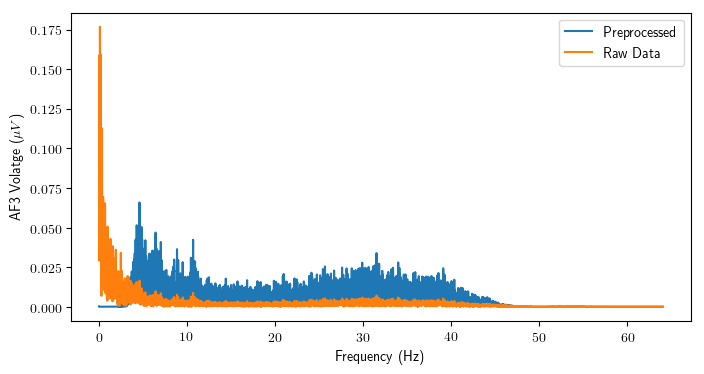
\includegraphics[width=\columnwidth]{tex/figures/filtering/AF3.png}
        \caption{AF3}
        \label{fig:filter:af3}
    \end{subfigure}
    \hfill
    \begin{subfigure}[t]{\columnwidth}
        \centering
        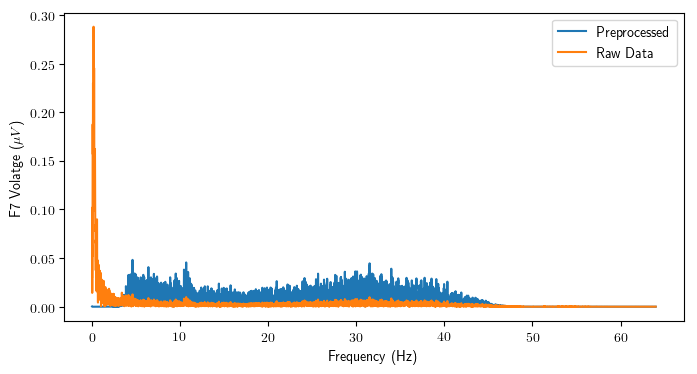
\includegraphics[width=\columnwidth]{tex/figures/filtering/F7.png}
        \caption{F7}
        \label{fig:filter:f7}
    \end{subfigure}
    \caption{Example filtering of EEG signal on sample 1 video 12}
    \label{fig:eeg}


    \begin{subfigure}[t]{\columnwidth}
        \centering
        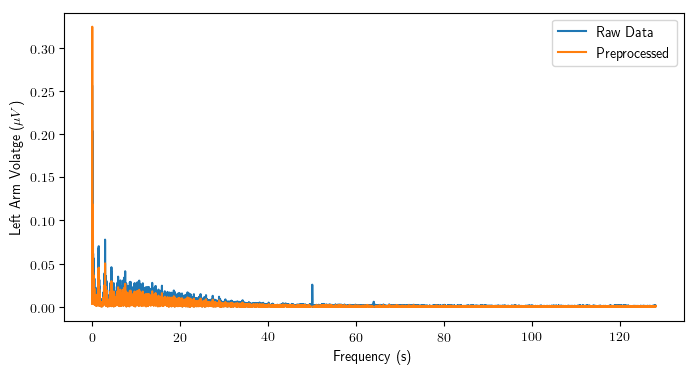
\includegraphics[width=\columnwidth]{tex/figures/filtering/ECG Left Arm.png}
        \caption{Left}
        \label{fig:filter:left}
    \end{subfigure}
    \hfill
    \begin{subfigure}[t]{\columnwidth}
        \centering
        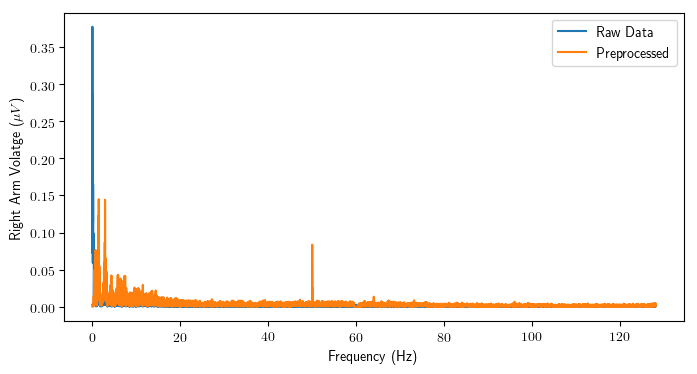
\includegraphics[width=\columnwidth]{tex/figures/filtering/ECG Right Arm.png}
        \caption{Right}
        \label{fig:filter:right}
    \end{subfigure}
    \caption{Example filtering of ECG signal on sample 1 video 12
             for the left and right arms}
    \label{fig:ecg}
\end{figure*}

\FloatBarrier
\section{Preprocessing}
We have applied 3 processing steps to our AMIGOS dataset;
signal filtering, [todo], and [todo].
In Figures \ref{fig:eeg} and \ref{fig:ecg}
we can see our filters applied to the EEG and ECG signals in the frequency domain.
For the EEG signal we followed the guideline set on the AMIGOS
website and applied a 4-45Hz bandpass filter \cite{AMIGOS:2018}.
We removed a significant amount of low frequency noise.
We can see that the preproccessed data results
in an slightly high amplitude than our original signal despite keeping the same shape.
Through experimental analysis we noticed that this was by a factor of 5.
For the ECG signal we applied a 0.5Hz highpass filter as noted in
\cite{SantamariaGranados:2019}
to remove baseline wander.
We also applied a bandstop filter with a 60Hz cutoff.
A small notch is visible in
Figures \ref{fig:filter:left} and \ref{fig:filter:right}.


\clearpage

    \section{Related Work}


    \bibliographystyle{IEEEtran}
    \bibliography{cite}

\end{document}
\endinput
